
\section{Software Design Component}

The software system we are designing will function as an information access portal (IAP) to Ontario's Electronic Health Record infrastructure. The main user of the system will be paramedics. Specifically, we plan to develop an application for use on both iOS and Android phones, that will allow paramedics to view a patients medical information. The information provided includes data such as allergies, medications and conditions that are useful to know in the case of an emergency. In the future, we hope the app can be extended to all areas of the medical profession as well as the general public.

It is important to note that we are not focused on acquiring medical information, as it will be available and stored by the province through the future EHR system. The focus of our software will be to access, process and present this information to a user.

\subsection{Software Technology}
In regards to application software, we will use the React Native Javascript framework to develop an Android, and iOS application concurrently. Additionally, the app will require a database to store patient information. For this, we plan on using Node.js to develop software that can access and process data from a MongoDB document database. The system will be modifiable, and compatible with accessing and retrieving information from Ontario's future EHR system.

\subsection{Functional Design}

There are a number of requirements the app is expected to meet in order to be useful to an EFR. Most importantly, the app should be compatible with the planned protocols and standards outlined in Ontario's eHealth blueprint, allowing it to be used in the future. These protocols include the HIAL and Health Level 7, an international standard for the exchange and handeling of medical information.

From a user perspective, the app will require a secure log-in for paramedics, a health card scanning system and screens to display and annotate electronic health record information. Additionally, it will need the ability to connect to a vitals-monitoring hardware device. An basic prototype of the app can be seen in figure~\ref{fig:app1}.

\begin{figure}[h]
  \centering
  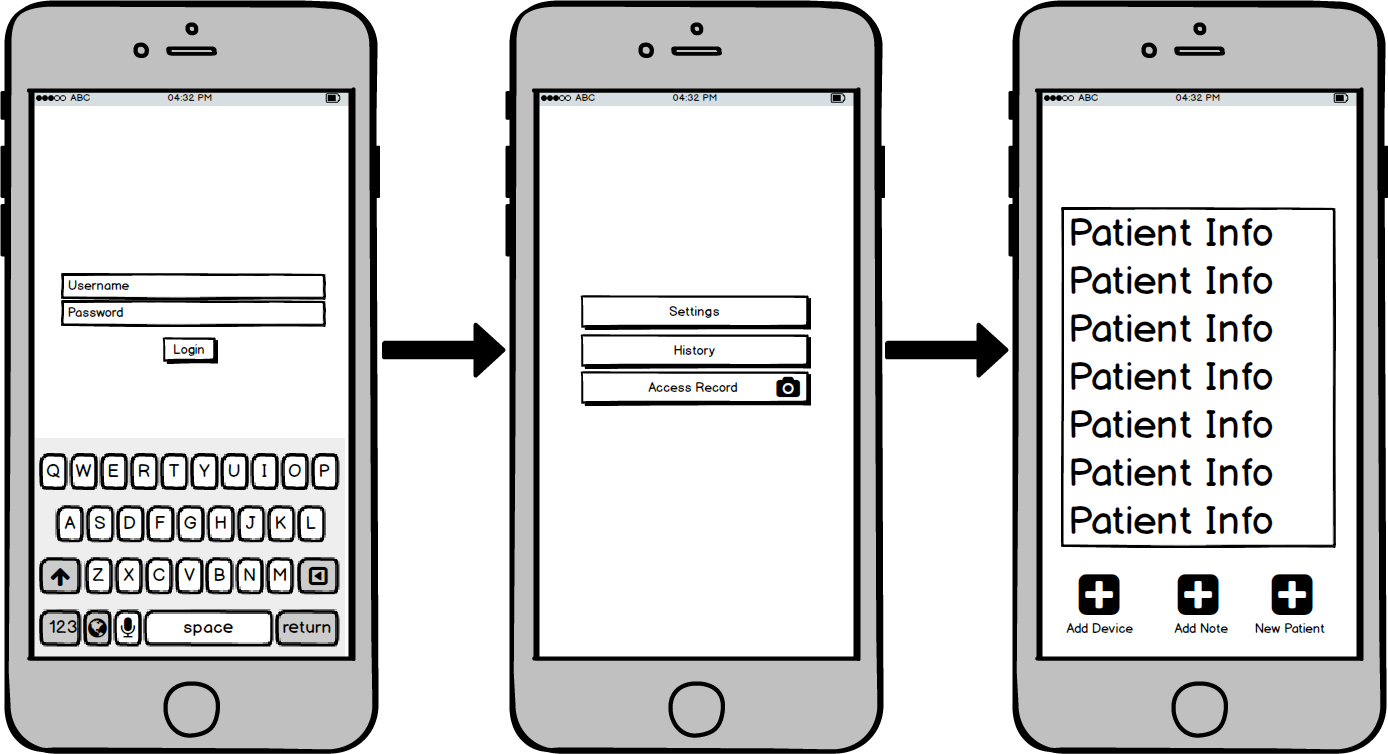
\includegraphics[width=\linewidth]{wireframe.png}
  \captionsetup{format=hang}
  \caption[Preliminary App Prototype]{A prototype of the information access portal application with the basic functional requirements, features and layout.}
  \label{fig:app1}
\end{figure}

As seen above, if a paramedic is using the app, they will be required to enter in a username and password, which will then bring them to a screen with access to the camera, call history, and settings. Accessing a record will require them to scan a health-card using the camera, or to enter the ID information manually. This will then bring them to the patients EMR, with information organized based on importance. The importance of information, and order in which it is presented will be determined in the future, most likely by discussing the app with EMRs. While responding to a call, the EMR will also have the ability to pair the app with a vitals tracker, logging important vitals information. This vitals information can be viewed in real-time, and stored for later use. If one or more patient's are present on the app the EMR will be able to see them all through different views and screens. The history screen will simply show what patients the paramedic has treated but will not allow the paramedic more access to their information once the paramedic has closed the patient's EHR.

\iffalse


The app's directory is laid out with different folders that depend on each other in different ways. The folders being screens, components, index, config and lib as seen in the hierarchy. The screens folder contains the layout of each different screen (ie. homepage, history, patient page), which are built using components from the components folder (button, title etc.). The index folder contains the locations of each of the screens and acts as a navigator. Lib contains a library of functions for collecting and fetching data. Config contains accesses index and creates each new page using screens and index.




In future versions the paramedic will be able to record information about the particular visit into the EHR, and will be able to view these additions on the history screen. In the future additions, the sensed data will also be stored and be visible in the EHR so medical personnel at a hospital or later at a doctor's visit will be able to view the patients vitals at the time of the paramedics visit.



\fi







\subsection{Non-Functional Design}
The app must have secure information storage and transmission by the standards outlined in the eHealth Blueprint. The app must have a cohesive look, including size and colour scheme in order to be easy to navigate. The app must be available in english and french. The app will be made so that the average paramedic is able to use it (assuming paramedics are males and females adults with above secondary education) and will use terms that are familiar to them.
The app must be able to run on Android and iOS devices that still recieve updates from their providers. The app must not have harsh colouring or flashing lights in order to prevent harm to the paramedics.
